\documentclass[11pt,a4paper]{article}
\usepackage{fontspec}
\setmainfont{DejaVuSerif}[Path=fonts/,Extension=.ttf,UprightFont=*,BoldFont=*-Bold,ItalicFont=*-Italic,BoldItalicFont=*-BoldItalic]
\setsansfont{DejaVuSans}[Path=fonts/,Extension=.ttf]
\setmonofont{DejaVuSansMono}[Path=fonts/,Extension=.ttf]
\usepackage[russian]{babel}
\usepackage[left=20mm,right=20mm,top=18mm,bottom=19mm]{geometry}
\usepackage{graphicx,booktabs,tabularx,array,xcolor,amsmath}
\usepackage{enumitem,fancyhdr,hyperref}
\definecolor{ink}{HTML}{162D46}
\definecolor{accent}{HTML}{245E8A}
\definecolor{muted}{HTML}{53616C}
\definecolor{pale}{HTML}{EFF4F8}
\hypersetup{colorlinks=true,urlcolor=accent,linkcolor=accent,pdftitle={LLM-агент для признаков и кандидатов: REES46 и OTTO}}
\setlength{\parindent}{0pt}
\setlength{\parskip}{3pt}
\raggedbottom
\setlength{\emergencystretch}{1em}
\makeatletter
\renewcommand\section{\@startsection{section}{1}{0pt}{2.0ex plus .5ex minus .2ex}{1.1ex plus .2ex}{\normalfont\large\bfseries\color{ink}}}
\makeatother
\renewcommand{\baselinestretch}{1.0}
\setlist[itemize]{leftmargin=15pt,itemsep=3pt,topsep=3pt}
\setlength{\tabcolsep}{4pt}
\renewcommand{\arraystretch}{1.16}
\newcolumntype{Y}{>{\raggedright\arraybackslash}X}
\pagestyle{fancy}
\fancyhf{}
\fancyhead[L]{\small\color{muted}T-Lab 2026 · RecSys · задача 1}
\fancyhead[R]{\small\color{muted}REES46 / OTTO}
\fancyfoot[C]{\small\thepage}
\renewcommand{\headrulewidth}{0pt}
\setlength{\headheight}{14pt}
\setlength{\headsep}{10pt}
\newcommand{\lead}[1]{\textbf{\color{ink}#1}}
\newcommand{\smallnote}[1]{{\small\color{muted}#1\par}}
\newcommand{\repo}[2]{\href{https://github.com/suprend/tlab-recsys-2026-task1/blob/3f8915dd5979d58709aa9442cdd79b79662dc6d1/#1}{#2}}
\begin{document}
\thispagestyle{empty}
{\small\color{muted}ОТБОР T-LAB 2026 \quad RECSYS · ЗАДАЧА 1\par}
\vspace{9pt}
{\LARGE\bfseries\color{ink}LLM-агент для признаков и кандидатов\par в рекомендательной системе\par}
\vspace{7pt}
{\large Проверка на REES46 и развитие решения OTTO\par}
\vspace{11pt}

\lead{Главный результат.} На REES46 совместный набор признаков агента и автоматических агрегатов улучшил базовую модель на данных более позднего периода примерно на \textbf{2\% по NDCG@20}. На OTTO агент менял также подбор товаров и за \textbf{три последовательные итерации} улучшил собственное решение.

\section*{1. Что мы поручили агенту}
Система сначала подбирает \textbf{кандидатов} (товары для рекомендации), затем модель ранжирования (\textbf{ранкер}) упорядочивает их по признакам: например, популярности товара и интересу пользователя к его категории.

Агент на основе языковой модели (LLM) получает описание данных и пишет SQL-запросы для расчёта новых признаков.

\begin{center}
\setlength{\fboxsep}{7pt}
\colorbox{pale}{\parbox{0.94\linewidth}{\centering\small
\textbf{Идея и SQL}\enspace$\longrightarrow$\enspace\textbf{Проверка и расчёт}\enspace$\longrightarrow$\enspace\textbf{Оценка качества}\\[4pt]
Результаты предыдущих предложений помогают выбрать следующую идею.
}}
\end{center}

На REES46 агент дополняет заданный набор признаков. На OTTO он может создавать ещё и источники кандидатов. Постановку, модель, ограничения и правила запуска задаём мы.

\section*{2. REES46: добавочные признаки к готовой базе}
\href{https://www.kaggle.com/datasets/mkechinov/ecommerce-behavior-data-from-multi-category-store}{REES46} содержит журнал просмотров, корзин и покупок одного многокатегорийного магазина. Доступны товар, категория, бренд, цена и сессия; названий товаров и профилей пользователей нет.

\lead{Задача.} В начале дня рекомендуем товары, с которыми пользователь не взаимодействовал в доступной истории. Целью считаем первое добавление такого товара в корзину или его покупку в следующие 24 часа. Покупки включены в цель, поскольку запись о предшествующем добавлении в корзину есть не всегда.

Запросом называем рекомендации одному пользователю в начале дня. В оценку входят запросы пользователей, активных за предыдущие 48 часов и совершивших хотя бы одно целевое действие в следующие сутки. Метрика NDCG@20 оценивает порядок первых двадцати рекомендаций. В её расчёт входят все целевые товары, включая не попавшие в кандидаты.

\lead{База.} Кандидатов подбирают по популярности, предпочтениям категорий и брендов, совместным просмотрам и переходам от просмотра к корзине или покупке. Их ранжирует градиентный бустинг CatBoost с функцией потерь Logloss. Он использует активность пользователя, популярность и конверсию товара, интерес к его категории и бренду, соответствие цены привычкам пользователя и связи с просмотренными товарами. На валидации проверяли настройки ранкера и способы выбора отрицательных примеров, затем условия обучения зафиксировали.

База подготовлена с помощью Claude Code и включает идеи ранней генерации признаков. Эксперимент проверяет, улучшают ли новые признаки эту систему, а не сравнивает способности LLM и человека.

\newpage
\section*{REES46: как проверяли и что получили}
Поиск проводили на данных 2019 года. Валидацию разделили на две части: на первой выбирали варианты, на второй, подтверждающей, проверяли, сохраняется ли улучшение.

\lead{Поиск и отбор.} За шесть раундов LLM-агент предложил 30 SQL-преобразований. Он видел схему, текущие признаки, оценки и ошибки прежних попыток, но не строки данных и целевые ответы. Признаки рассчитывали только по прошлым событиям. Для проверки каждого предложения модель переобучали с ранее принятыми и новыми признаками. В каждом раунде принимали лучшее предложение, если прирост NDCG@20 превышал порог отбора 0.0005, а доверительный интервал лежал выше нуля в двух запусках обучения. Так отобрали одно предложение с двумя признаками: близость кандидата к товарам, к которым пользователь возвращался в нескольких сессиях. Число раундов задавал человек.

Для контроля использовали фиксированную сетку агрегатов (в коде \textbf{DFS}). Она без LLM перебирает заданные окна и типы событий, рассчитывая статистики пользователя, товара, категории и бренда. Её признаки отбирали по важности на обучающих данных.

\lead{Проверка на новом периоде.} После первоначального теста на данных 2019 года возникла гипотеза: добавить все признаки агента и DFS без отбора. Сначала её проверили на валидации 2019, затем на новом тесте в феврале 2020. Перед тестом модели переобучили на предшествующей истории 2020 года, сохранив настройки и правила расчёта признаков из 2019.

Для вариантов в таблице совпадали разбиение, кандидаты, доступная история и настройки модели. Полный набор агента и DFS расширяет базу с 80 до 274 признаков. В таблице приведено среднее по двум запускам обучения с разными начальными состояниями генератора случайных чисел (seed).

\lead{Критерий успеха.} До открытия теста для полного набора потребовали абсолютный прирост NDCG@20 не меньше 0.0015 и положительную нижнюю границу 95\%-го доверительного интервала в обоих запусках. Интервалы получены повторными выборками запросов и не отражают разброс новых запусков самого агента.

\smallnote{Тест: 14--29 февраля 2020, около 98 тыс. запросов; 27--28 февраля исключены по заранее заданному правилу аномального падения числа событий. Обучение перед тестом: 15 января -- 13 февраля.}

\begin{center}\small
\begin{tabularx}{\linewidth}{@{}Yrr@{}}
\toprule
\textbf{Вариант на тесте 2020} & \textbf{NDCG@20} & \textbf{Изменение}\\
\midrule
База & 0.1462 & база\\
База + отобранное предложение агента & 0.1470 & +0.0008\\
База + отобранные признаки DFS & 0.1459 & $-0.0003$\\
\textbf{База + весь набор агента и DFS} & \textbf{0.1492} & \textbf{+0.0030}\\
Автоматические признаки вместо ручных & 0.1451 & $-0.0011$\\
\bottomrule
\end{tabularx}
\end{center}
\smallnote{Изменение относительно базы. Разности посчитаны до округления. При замене ручных признаков сохранены позиции товаров в списках кандидатов.}

\lead{Полный набор прошёл заранее заданную проверку.}

\smallnote{Прирост и 95\%-й интервал по запускам: $+0.0031\;[+0.0025; +0.0036]$ и $+0.0029\;[+0.0023; +0.0035]$.}

\lead{Что не сработало.} Эффект отобранного предложения ослаб на подтверждающей части. На новом тесте выигрыш остался ниже практического порога 0.001 для отдельного предложения. Полная замена ручных признаков немного уступила базе; отдельно этот вариант не настраивали.

\smallnote{В последующих проверках прироста полного набора относительно базы интервалы остались выше нуля при группировке запросов отдельно по пользователям и дням; выигрыш сохранялся и при исключении любого одного дня. Дневная оценка ограничена 14 днями; совместные зависимости по пользователям и дням не учитывались. В обоих запусках выросла и полнота рекомендаций (Recall@20). На запросах с покупками выросли NDCG@20 и Recall@20 только купленных товаров. Интервалы этих приростов при группировке по пользователям также выше нуля.}

\lead{Последующие проверки на валидации.} Перемешивание автоматических признаков между строками внутри дня сохраняло их число и распределения, но убирало выигрыш. Полный набор агента улучшал базу без DFS; интервалы добавочного эффекта DFS на валидации обоих периодов включали ноль.

% AGENT_TEST_ABLATION
\lead{Дополнительный разбор теста.} Отдельно обучили вариант «база + весь набор агента без DFS» с теми же настройками и двумя seed. Средний NDCG@20 составил \textbf{0.1491} против 0.1462 у базы, прирост около \textbf{2.0\%}. В обоих запусках 95\%-е интервалы прироста с группировкой по пользователям выше нуля. Оба интервала добавочного эффекта DFS включают ноль; это не доказывает равенства вариантов. Такой разбор уже просмотренного теста не является независимой итоговой проверкой.

\newpage
\section*{3. OTTO: три улучшения агентной системы}
В \href{https://github.com/otto-de/recsys-dataset/blob/main/KAGGLE.md}{задаче Kaggle OTTO} по началу сессии нужно предсказать товар следующего клика и товары последующих добавлений в корзину и заказов. Итоговая метрика объединяет полноту первых двадцати рекомендаций для этих действий. \textbf{Private score} показывает качество на части теста Kaggle, метки которой наша система не использовала. После каждой отправки предсказаний Kaggle показывал значение этой метрики.

\lead{Как работает агент.} Он создаёт таблицы связей между товарами для подбора кандидатов и расчёта признаков. Например, предлагает товары, которые добавляли в корзину или заказывали вместе, либо товары, к которым переходили после похожих просмотров.

Первый запуск агента усилил простую систему на основе истории сессии и популярности. Затем мы изменили обучение ранкера, сохранив предложенные агентом источники кандидатов и признаки; так получили OTTO-2. Следующие три итерации запускал человек. \textbf{Способ обучения ранкера оставался прежним}, а агент развивал набор кандидатов и признаков.

\begin{center}\small
\begin{tabularx}{\linewidth}{@{}p{22mm}Y@{}}
\toprule
\textbf{Итерация} & \textbf{Что изменилось}\\
\midrule
Первая & Новый запуск агента с расширенными лимитами поиска. Добавлены источники кандидатов и признаки.\\
Вторая & Агент дополнил предыдущий набор новыми источниками кандидатов и признаками.\\
Третья & Агент добавил только признаки. Кандидаты остались прежними.\\
\bottomrule
\end{tabularx}
\end{center}

\begin{center}
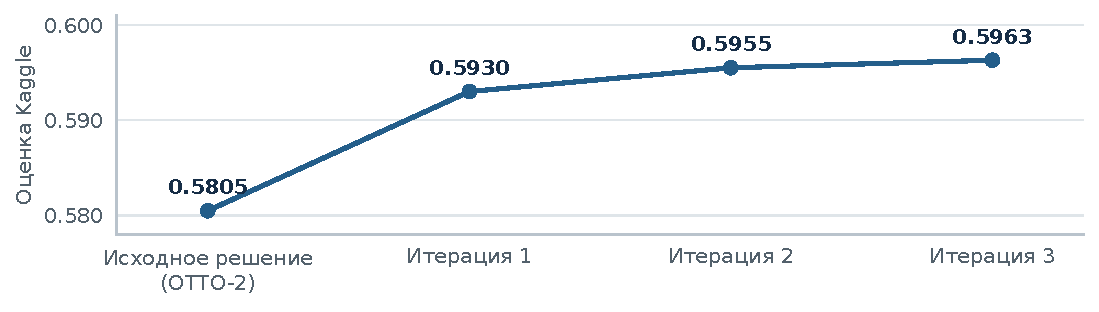
\includegraphics[width=0.98\linewidth]{images/otto-iterations.pdf}
\end{center}
\smallnote{Ось показана не от нуля.}

\lead{Результат.} Три итерации дали суммарно около \textbf{2.7\%} к private относительно OTTO-2. Каждый шаг улучшал оценку на локальной валидации и private.

Первые два шага меняли одновременно кандидатов и признаки, поэтому их вклады не разделены. В числе предложенных идей были переходы с учётом типа события, похожие исторические сессии и оценка длительности просмотра по промежуткам между событиями. Польза каждого отдельного признака не измерялась.


\newpage
\section*{4. Границы результатов и выводы}
В этих экспериментах автоматическая генерация помогла расширить готовую систему. На REES46 полная замена ручных признаков уступила базе. Повторяемость улучшений при независимых повторах поиска от одной и той же базы не проверена ни на REES46, ни на OTTO.

\lead{REES46.} Эффект проверен в одном магазине и на одном новом тестовом периоде. Устойчивость результата на других наборах данных не установлена.

\begin{itemize}
\item \textbf{Выбор по валидации.} Подтверждающая часть не была полностью изолирована: её оценки были видны в ранних прогонах. Правила принятия настроек базы и предложений агента различались; выбранное предложение вошло в тест 2019, хотя на подтверждающей части выигрыш не подтвердился. Последнее уточнение плана 2020 внесено после просмотра валидации, без изменения вариантов и порогов теста.
\item \textbf{Настройка базы.} Настройки проверяли ограниченным набором вариантов; полного совместного поиска и сравнения при равных вычислительных бюджетах не проводили. Порог для отдельного предложения основан на разбросе между запусками обучения и не является универсальной границей полезности.
\item \textbf{Доступность истории.} Сравнивали признаки по полному журналу и по истории до момента прогноза. Найденную ошибку доступности кода категории исправили до обучения моделей 2020. Возможность обойти ограничения доступа к данным устранили до запуска агента. Эти проверки уменьшают риск утечек, но не доказывают отсутствие всех возможных ошибок.
\end{itemize}

\lead{OTTO.} Оценки использовались в ходе поиска, поэтому результат не равнозначен одноразовой итоговой проверке.

\begin{itemize}
\item \textbf{Повторное использование оценок.} Локальную валидацию многократно использовали при выборе вариантов. На Kaggle отправили девять файлов с предсказаниями; после достижения намеченной private-оценки продолжили ещё две итерации. Критерий пригодности простой базы также изменили после просмотра локальных оценок.
\item \textbf{Доступность информации.} В выбранном режиме Kaggle допустимо использовать события других сессий после момента прогноза. Такой эксперимент не проверяет строгую постановку «только прошлое» из задания.
\item \textbf{Контроль и новизна.} Превосходство над сильной ручной системой при одинаковых кандидатах не проверено. LLM могла воспроизводить известные решения соревнования; новизну предложений мы не установили.
\end{itemize}

\lead{Затраты.} Суммарное время вычислительных этапов агента на REES46 составило около пяти часов, из них около 6\% заняла работа LLM. Основное время ушло на переобучение моделей для проверки идей. В повторе 2020 чтение готовых признаков, обучение и оценка в двух запусках суммарно заняли около 21 минуты для базы и 33 минут для совместного набора агента и DFS. Это один замер без учёта расчёта признаков. В OTTO проверку утечек пришлось разбить на части: для расчёта на всей выборке не хватало памяти.

\smallskip
\small
\lead{Код и воспроизведение.} \href{https://github.com/suprend/tlab-recsys-2026-task1}{Репозиторий проекта}; инструкции для \href{https://github.com/suprend/tlab-recsys-2026-task1/blob/main/docs/task1-reproduce.md}{REES46} и \href{https://github.com/suprend/tlab-recsys-2026-task1/blob/main/docs/otto-reproduce.md}{OTTO}; \repo{task1/runs/replication-2020/test.json}{числа теста 2020} и \repo{docs/otto3-run/otto3-kaggle-scores.csv}{оценки предсказаний OTTO}. Сырые данные, тяжёлые артефакты и расширенная проверка разброса случайных запусков находятся вне Git.

\lead{Участие ИИ.} Автор выбирал направления и разрешал запуски; Claude Code проектировал значительную часть системы и написал код. Генерацию SQL исследовали как отдельный компонент. Ревью другими экземплярами LLM не исключает общих ошибок модели.
\end{document}
